
\subsection{Work Breakdown Structure}

The team was categorized into different groups of responsibilities with dedicated leaders who reported to and coordinated with the Project Manager. Leadership was organized on a rotational basis when the need arose. The formation of these divisions constituted a work breakdown structure which is illustrated in Figure \ref{fig:work-breakdown-structure}.

The Management was composed of a Project Manager and a Deputy Project Manager, both acted as Systems Engineer and managing overall implementation of the project. The Project Manager was responsible for establishing and overseeing product development cycle; coordinating between different teams, project stakeholders, and documentation efforts; outreach and public relations; Fundraising; monitoring and reporting; system integration; and quality assurance. Once all subsystems had been assembled, the Project Manager was also responsible for overseeing the integration processes leading to the final experiment setup and put emphasis on leading quality assurance integration testing efforts. The Deputy Project Manager assisted the Project Manager in all management duties in a manner that ensured replaceability when necessary.

The Scientific Division was responsible for defining experiment parameters; data analysis; interpreting and documenting measurements; researching previous CAC experiments for comparative analysis purposes; evaluating the reliability of the proposed AAC sampling system; conducting measurements of collected samples; documenting and publishing findings; defining experiment parameters; contacting researchers or institutions working on similar projects; exploring potential partnership with researchers and institutions; documenting and publishing findings.

The Mechanical Division was responsible for designing or redesigning cost-effective mechanical devices using analysis and computer-aided design; producing details of specifications and outline designs; overseeing the manufacturing process for the devices; identifying material and component suppliers; developing and testing prototypes of designed devices; analyzing test results and changing the design as needed; and integrating and assembling final design.

The Electrical Division was responsible for designing and implementing cost-effective circuitry using analysis and computer-aided design; producing details of specifications and outline designs; developing, testing, and evaluating theoretical designs; identifying material as well as component suppliers; reviewing and testing proposed designs; recommending modifications following prototype test results; and assembling designed circuitry.

The Software Division was responsible for gathering software requirements; formalizing software specifications; drafting architecture design; leading software implementation efforts; leading quality assurance and testing efforts; enforcing software testing best practices such as continuous integration testing and regression testing; reviewing requirements and specifications in order to foresee potential issues; providing input for functional requirements; advising on design; formalizing test cases; tracking defects and ensuring their resolution; facilitating code review sessions; and supporting software implementation efforts.

The Thermal Division was responsible for ensuring thermal regulation of the payload as per operational requirements of all experiment components; evaluating designs against thermal simulation and propose improvements; managing against mechanical design and electrical power limitations towards providing passive and active thermal control systems.

\begin{landscape}
\begin{figure}[p]
    \begin{align*}
        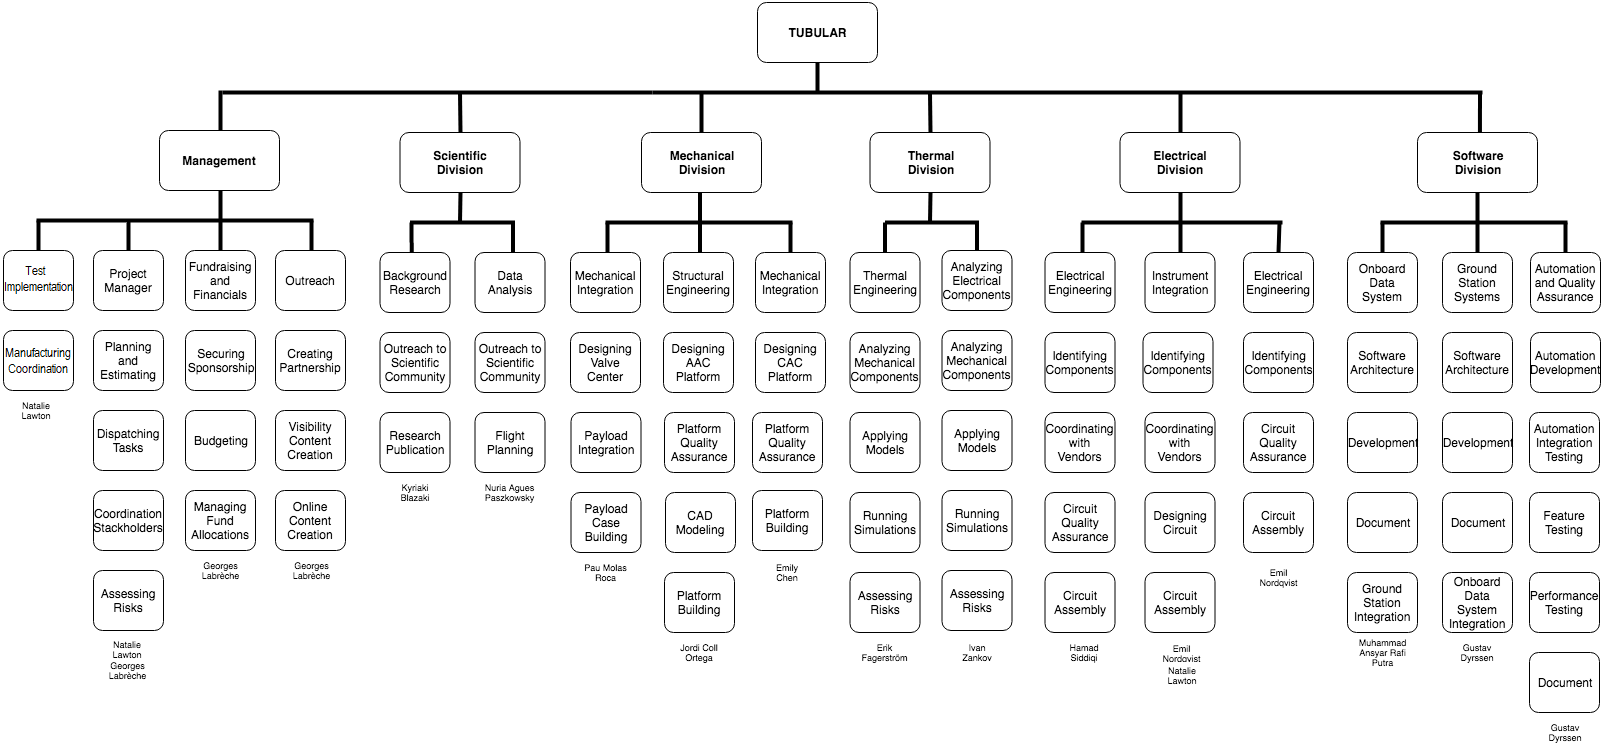
\includegraphics[width=24cm]{3-project-planning/img/work-breakdown-structure-updated.png}
    \end{align*}
    \caption{Work Breakdown Structure.}\label{fig:work-breakdown-structure}
\end{figure}
\end{landscape}